\documentclass{standalone}
\usepackage{tikz}
\usetikzlibrary{patterns, positioning}

\begin{document}
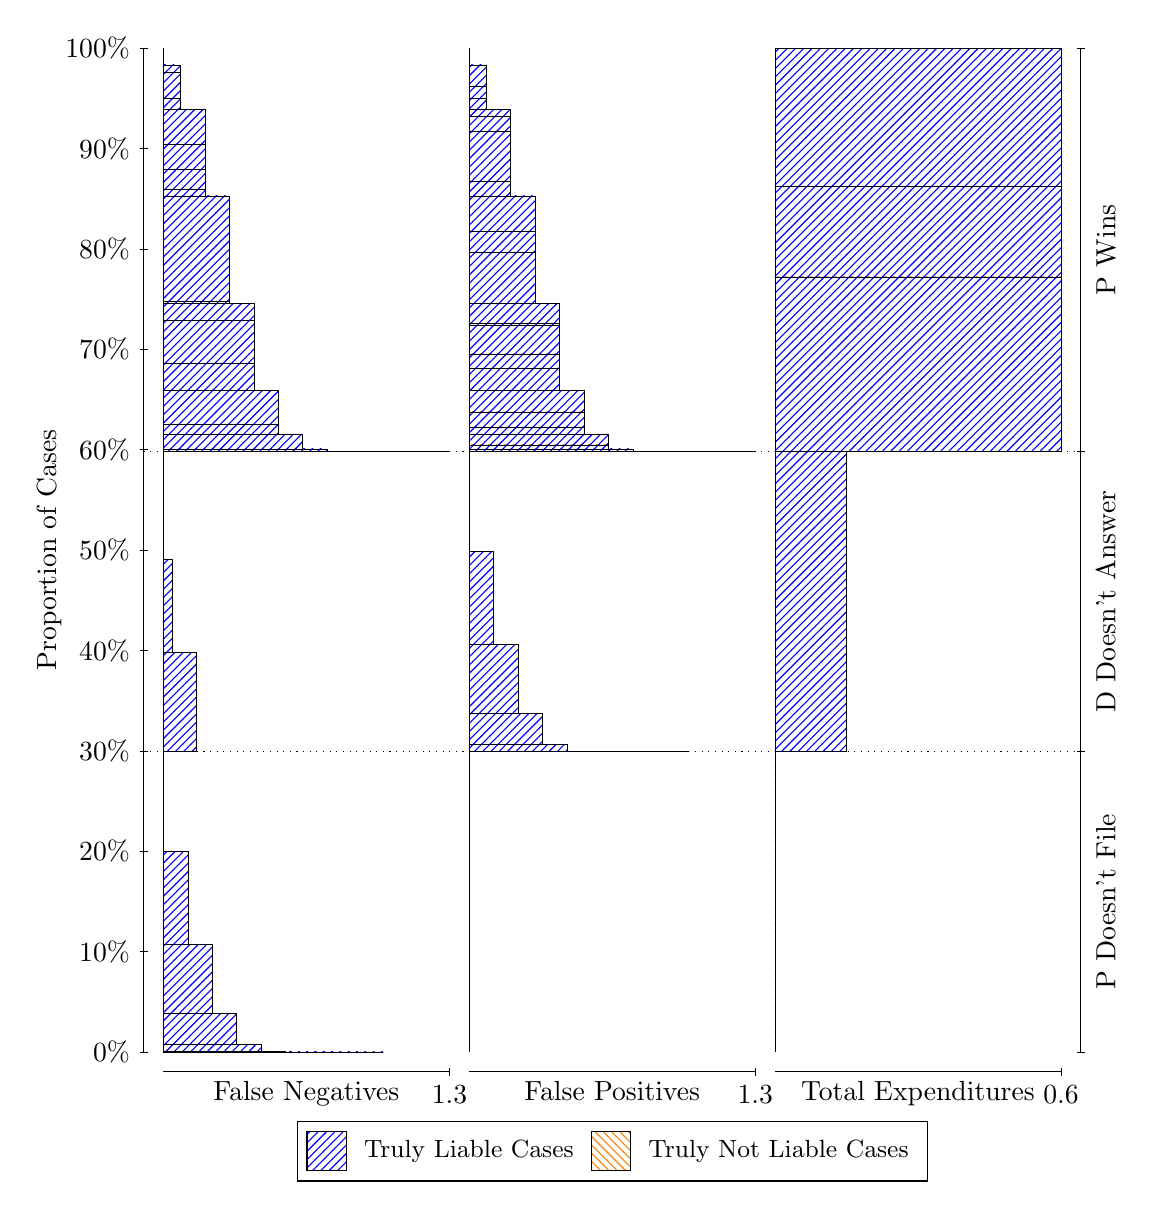
\begin{tikzpicture}
\draw[black, very thin] (1.5,1.75) -- (1.5,14.5);
\node[rotate=90, anchor=center] at (0.3, 8.125) {Proportion of Cases};
\draw[black, very thin] (1.45,1.75) -- (1.55,1.75);
\node[anchor=east] at (1.45, 1.75) {0\%};
\draw[black, very thin] (1.45,3.025) -- (1.55,3.025);
\node[anchor=east] at (1.45, 3.025) {10\%};
\draw[black, very thin] (1.45,4.3) -- (1.55,4.3);
\node[anchor=east] at (1.45, 4.3) {20\%};
\draw[black, very thin] (1.45,5.575) -- (1.55,5.575);
\node[anchor=east] at (1.45, 5.575) {30\%};
\draw[black, very thin] (1.45,6.85) -- (1.55,6.85);
\node[anchor=east] at (1.45, 6.85) {40\%};
\draw[black, very thin] (1.45,8.125) -- (1.55,8.125);
\node[anchor=east] at (1.45, 8.125) {50\%};
\draw[black, very thin] (1.45,9.4) -- (1.55,9.4);
\node[anchor=east] at (1.45, 9.4) {60\%};
\draw[black, very thin] (1.45,10.675) -- (1.55,10.675);
\node[anchor=east] at (1.45, 10.675) {70\%};
\draw[black, very thin] (1.45,11.95) -- (1.55,11.95);
\node[anchor=east] at (1.45, 11.95) {80\%};
\draw[black, very thin] (1.45,13.225) -- (1.55,13.225);
\node[anchor=east] at (1.45, 13.225) {90\%};
\draw[black, very thin] (1.45,14.5) -- (1.55,14.5);
\node[anchor=east] at (1.45, 14.5) {100\%};

\draw[black, very thin] (13.4,1.75) -- (13.4,14.5);
\draw[black, very thin] (13.35,1.75) -- (13.45,1.75);
\node[anchor=west] at (13.35, 1.75) {};
\draw[black, very thin] (13.35,5.563) -- (13.45,5.563);
\node[anchor=west] at (13.35, 5.563) {};
\draw[black, very thin] (13.35,9.3748) -- (13.45,9.3748);
\node[anchor=west] at (13.35, 9.3748) {};
\draw[black, very thin] (13.35,14.5) -- (13.45,14.5);
\node[anchor=west] at (13.35, 14.5) {};

\draw[black, very thin, pattern color=blue, pattern=north east lines] (1.75,1.75) rectangle (4.5449,1.75);
\draw[black, very thin, pattern color=blue, pattern=north east lines] (1.75,1.75) rectangle (4.2343,1.75);
\draw[black, very thin, pattern color=blue, pattern=north east lines] (1.75,1.75) rectangle (3.9238,1.75);
\draw[black, very thin, pattern color=blue, pattern=north east lines] (1.75,1.75) rectangle (3.6132,1.7503);
\draw[black, very thin, pattern color=blue, pattern=north east lines] (1.75,1.7503) rectangle (3.3027,1.7582);
\draw[black, very thin, pattern color=blue, pattern=north east lines] (1.75,1.7582) rectangle (2.9922,1.8434);
\draw[black, very thin, pattern color=blue, pattern=north east lines] (1.75,1.8434) rectangle (2.6816,2.2366);
\draw[black, very thin, pattern color=blue, pattern=north east lines] (1.75,2.2366) rectangle (2.3711,3.1157);
\draw[black, very thin, pattern color=blue, pattern=north east lines] (1.75,3.1157) rectangle (2.0605,4.2995);
\draw[black, very thin, pattern color=orange, pattern=north west lines] (1.75,4.2995) rectangle (1.75,4.2995);
\draw[black, very thin, pattern color=blue, pattern=north east lines] (1.75,4.2995) rectangle (1.75,5.563);
\draw[black, very thin, pattern color=blue, pattern=north east lines] (1.75,5.563) rectangle (2.1692,6.8266);
\draw[black, very thin, pattern color=blue, pattern=north east lines] (1.75,6.8266) rectangle (1.8587,8.0103);
\draw[black, very thin, pattern color=orange, pattern=north west lines] (1.75,8.0103) rectangle (1.75,8.0103);
\draw[black, very thin, pattern color=blue, pattern=north east lines] (1.75,8.0103) rectangle (1.75,9.3748);
\draw[black, very thin, pattern color=blue, pattern=north east lines] (1.75,9.3748) rectangle (5.3833,9.3748);
\draw[black, very thin, pattern color=blue, pattern=north east lines] (1.75,9.3748) rectangle (5.0728,9.3748);
\draw[black, very thin, pattern color=blue, pattern=north east lines] (1.75,9.3748) rectangle (4.7623,9.3748);
\draw[black, very thin, pattern color=blue, pattern=north east lines] (1.75,9.3748) rectangle (4.4517,9.3749);
\draw[black, very thin, pattern color=blue, pattern=north east lines] (1.75,9.3749) rectangle (4.4517,9.375);
\draw[black, very thin, pattern color=blue, pattern=north east lines] (1.75,9.375) rectangle (4.1412,9.377);
\draw[black, very thin, pattern color=blue, pattern=north east lines] (1.75,9.377) rectangle (4.1412,9.3782);
\draw[black, very thin, pattern color=blue, pattern=north east lines] (1.75,9.3782) rectangle (3.8306,9.4104);
\draw[black, very thin, pattern color=blue, pattern=north east lines] (1.75,9.4104) rectangle (3.5201,9.5885);
\draw[black, very thin, pattern color=blue, pattern=north east lines] (1.75,9.5885) rectangle (3.2095,9.7198);
\draw[black, very thin, pattern color=blue, pattern=north east lines] (1.75,9.7198) rectangle (3.2095,10.155);
\draw[black, very thin, pattern color=blue, pattern=north east lines] (1.75,10.155) rectangle (2.899,10.159);
\draw[black, very thin, pattern color=blue, pattern=north east lines] (1.75,10.159) rectangle (2.899,10.496);
\draw[black, very thin, pattern color=blue, pattern=north east lines] (1.75,10.496) rectangle (2.899,11.044);
\draw[black, very thin, pattern color=blue, pattern=north east lines] (1.75,11.044) rectangle (2.899,11.254);
\draw[black, very thin, pattern color=blue, pattern=north east lines] (1.75,11.254) rectangle (2.5885,11.287);
\draw[black, very thin, pattern color=blue, pattern=north east lines] (1.75,11.287) rectangle (2.5885,12.621);
\draw[black, very thin, pattern color=blue, pattern=north east lines] (1.75,12.621) rectangle (2.2779,12.708);
\draw[black, very thin, pattern color=blue, pattern=north east lines] (1.75,12.708) rectangle (2.2779,12.958);
\draw[black, very thin, pattern color=blue, pattern=north east lines] (1.75,12.958) rectangle (2.2779,13.283);
\draw[black, very thin, pattern color=blue, pattern=north east lines] (1.75,13.283) rectangle (2.2779,13.72);
\draw[black, very thin, pattern color=blue, pattern=north east lines] (1.75,13.72) rectangle (1.9674,13.865);
\draw[black, very thin, pattern color=blue, pattern=north east lines] (1.75,13.865) rectangle (1.9674,14.188);
\draw[black, very thin, pattern color=blue, pattern=north east lines] (1.75,14.188) rectangle (1.9674,14.286);
\draw[black, very thin, pattern color=orange, pattern=north west lines] (1.75,14.286) rectangle (1.75,14.286);
\draw[black, very thin, pattern color=blue, pattern=north east lines] (1.75,14.286) rectangle (1.75,14.5);
\draw[black, very thin, pattern color=orange, pattern=north west lines] (5.6333,1.75) rectangle (5.6333,1.75);
\draw[black, very thin, pattern color=blue, pattern=north east lines] (5.6333,1.75) rectangle (5.6333,5.563);
\draw[black, very thin, pattern color=orange, pattern=north west lines] (5.6333,5.563) rectangle (8.4282,5.563);
\draw[black, very thin, pattern color=blue, pattern=north east lines] (5.6333,5.563) rectangle (8.4282,5.563);
\draw[black, very thin, pattern color=blue, pattern=north east lines] (5.6333,5.563) rectangle (8.1177,5.563);
\draw[black, very thin, pattern color=blue, pattern=north east lines] (5.6333,5.563) rectangle (7.8071,5.563);
\draw[black, very thin, pattern color=blue, pattern=north east lines] (5.6333,5.563) rectangle (7.4966,5.5632);
\draw[black, very thin, pattern color=blue, pattern=north east lines] (5.6333,5.5632) rectangle (7.186,5.5706);
\draw[black, very thin, pattern color=blue, pattern=north east lines] (5.6333,5.5706) rectangle (6.8755,5.6552);
\draw[black, very thin, pattern color=blue, pattern=north east lines] (5.6333,5.6552) rectangle (6.565,6.0483);
\draw[black, very thin, pattern color=blue, pattern=north east lines] (5.6333,6.0483) rectangle (6.2544,6.9275);
\draw[black, very thin, pattern color=blue, pattern=north east lines] (5.6333,6.9275) rectangle (5.9439,8.1112);
\draw[black, very thin, pattern color=blue, pattern=north east lines] (5.6333,8.1112) rectangle (5.6333,9.3748);
\draw[black, very thin, pattern color=orange, pattern=north west lines] (5.6333,9.3748) rectangle (9.2667,9.3748);
\draw[black, very thin, pattern color=blue, pattern=north east lines] (5.6333,9.3748) rectangle (9.2667,9.3748);
\draw[black, very thin, pattern color=orange, pattern=north west lines] (5.6333,9.3748) rectangle (8.9561,9.3748);
\draw[black, very thin, pattern color=blue, pattern=north east lines] (5.6333,9.3748) rectangle (8.9561,9.3748);
\draw[black, very thin, pattern color=blue, pattern=north east lines] (5.6333,9.3748) rectangle (8.6456,9.3748);
\draw[black, very thin, pattern color=orange, pattern=north west lines] (5.6333,9.3748) rectangle (8.6456,9.3748);
\draw[black, very thin, pattern color=blue, pattern=north east lines] (5.6333,9.3748) rectangle (8.6456,9.3748);
\draw[black, very thin, pattern color=blue, pattern=north east lines] (5.6333,9.3748) rectangle (8.335,9.3749);
\draw[black, very thin, pattern color=blue, pattern=north east lines] (5.6333,9.3749) rectangle (8.335,9.375);
\draw[black, very thin, pattern color=orange, pattern=north west lines] (5.6333,9.375) rectangle (8.335,9.375);
\draw[black, very thin, pattern color=blue, pattern=north east lines] (5.6333,9.375) rectangle (8.335,9.375);
\draw[black, very thin, pattern color=orange, pattern=north west lines] (5.6333,9.375) rectangle (8.0245,9.375);
\draw[black, very thin, pattern color=blue, pattern=north east lines] (5.6333,9.375) rectangle (8.0245,9.3775);
\draw[black, very thin, pattern color=blue, pattern=north east lines] (5.6333,9.3775) rectangle (8.0245,9.378);
\draw[black, very thin, pattern color=blue, pattern=north east lines] (5.6333,9.378) rectangle (8.0245,9.3782);
\draw[black, very thin, pattern color=orange, pattern=north west lines] (5.6333,9.3782) rectangle (7.714,9.3782);
\draw[black, very thin, pattern color=blue, pattern=north east lines] (5.6333,9.3782) rectangle (7.714,9.4068);
\draw[black, very thin, pattern color=blue, pattern=north east lines] (5.6333,9.4068) rectangle (7.714,9.4104);
\draw[black, very thin, pattern color=blue, pattern=north east lines] (5.6333,9.4104) rectangle (7.4034,9.46);
\draw[black, very thin, pattern color=orange, pattern=north west lines] (5.6333,9.46) rectangle (7.4034,9.46);
\draw[black, very thin, pattern color=blue, pattern=north east lines] (5.6333,9.46) rectangle (7.4034,9.5885);
\draw[black, very thin, pattern color=blue, pattern=north east lines] (5.6333,9.5885) rectangle (7.0929,9.6872);
\draw[black, very thin, pattern color=blue, pattern=north east lines] (5.6333,9.6872) rectangle (7.0929,9.8781);
\draw[black, very thin, pattern color=orange, pattern=north west lines] (5.6333,9.8781) rectangle (7.0929,9.8781);
\draw[black, very thin, pattern color=blue, pattern=north east lines] (5.6333,9.8781) rectangle (7.0929,10.155);
\draw[black, very thin, pattern color=blue, pattern=north east lines] (5.6333,10.155) rectangle (6.7823,10.427);
\draw[black, very thin, pattern color=blue, pattern=north east lines] (5.6333,10.427) rectangle (6.7823,10.615);
\draw[black, very thin, pattern color=orange, pattern=north west lines] (5.6333,10.615) rectangle (6.7823,10.615);
\draw[black, very thin, pattern color=blue, pattern=north east lines] (5.6333,10.615) rectangle (6.7823,10.982);
\draw[black, very thin, pattern color=blue, pattern=north east lines] (5.6333,10.982) rectangle (6.7823,11.004);
\draw[black, very thin, pattern color=blue, pattern=north east lines] (5.6333,11.004) rectangle (6.7823,11.254);
\draw[black, very thin, pattern color=blue, pattern=north east lines] (5.6333,11.254) rectangle (6.4718,11.906);
\draw[black, very thin, pattern color=orange, pattern=north west lines] (5.6333,11.906) rectangle (6.4718,11.906);
\draw[black, very thin, pattern color=blue, pattern=north east lines] (5.6333,11.906) rectangle (6.4718,12.171);
\draw[black, very thin, pattern color=blue, pattern=north east lines] (5.6333,12.171) rectangle (6.4718,12.621);
\draw[black, very thin, pattern color=blue, pattern=north east lines] (5.6333,12.621) rectangle (6.1613,12.808);
\draw[black, very thin, pattern color=blue, pattern=north east lines] (5.6333,12.808) rectangle (6.1613,13.445);
\draw[black, very thin, pattern color=blue, pattern=north east lines] (5.6333,13.445) rectangle (6.1613,13.632);
\draw[black, very thin, pattern color=blue, pattern=north east lines] (5.6333,13.632) rectangle (6.1613,13.72);
\draw[black, very thin, pattern color=blue, pattern=north east lines] (5.6333,13.72) rectangle (5.8507,13.865);
\draw[black, very thin, pattern color=blue, pattern=north east lines] (5.6333,13.865) rectangle (5.8507,14.01);
\draw[black, very thin, pattern color=blue, pattern=north east lines] (5.6333,14.01) rectangle (5.8507,14.286);
\draw[black, very thin, pattern color=blue, pattern=north east lines] (5.6333,14.286) rectangle (5.6333,14.5);
\draw[black, very thin, pattern color=orange, pattern=north west lines] (9.5167,1.75) rectangle (9.5167,1.75);
\draw[black, very thin, pattern color=blue, pattern=north east lines] (9.5167,1.75) rectangle (9.5167,5.563);
\draw[black, very thin, pattern color=orange, pattern=north west lines] (9.5167,5.563) rectangle (10.425,5.563);
\draw[black, very thin, pattern color=blue, pattern=north east lines] (9.5167,5.563) rectangle (10.425,9.3748);
\draw[black, very thin, pattern color=orange, pattern=north west lines] (9.5167,9.3748) rectangle (13.15,9.3748);
\draw[black, very thin, pattern color=blue, pattern=north east lines] (9.5167,9.3748) rectangle (13.15,11.593);
\draw[black, very thin, pattern color=orange, pattern=north west lines] (9.5167,11.593) rectangle (13.15,11.593);
\draw[black, very thin, pattern color=blue, pattern=north east lines] (9.5167,11.593) rectangle (13.15,12.738);
\draw[black, very thin, pattern color=orange, pattern=north west lines] (9.5167,12.738) rectangle (13.15,12.738);
\draw[black, very thin, pattern color=blue, pattern=north east lines] (9.5167,12.738) rectangle (13.15,14.5);
\draw[black, dotted] (1.5,5.563) -- (13.4,5.563);
\draw[black, dotted] (1.5,9.3748) -- (13.4,9.3748);
\draw[black, very thin] (1.75,1.5) -- (5.3833,1.5);
\node[anchor=north] at (3.5667, 1.5) {False Negatives};
\draw[black, very thin] (5.3833,1.45) -- (5.3833,1.55);
\node[anchor=north] at (5.3833, 1.45) {1.3};

\draw[black, very thin] (5.6333,1.5) -- (9.2667,1.5);
\node[anchor=north] at (7.45, 1.5) {False Positives};
\draw[black, very thin] (9.2667,1.45) -- (9.2667,1.55);
\node[anchor=north] at (9.2667, 1.45) {1.3};

\draw[black, very thin] (9.5167,1.5) -- (13.15,1.5);
\node[anchor=north] at (11.333, 1.5) {Total Expenditures};
\draw[black, very thin] (13.15,1.45) -- (13.15,1.55);
\node[anchor=north] at (13.15, 1.45) {0.6};

\node[black, centered, rotate=90] at (13.72, 3.6565) {P Doesn't File};
\node[black, centered, rotate=90] at (13.72, 7.4689) {D Doesn't Answer};
\node[black, centered, rotate=90] at (13.72, 11.937) {P Wins};

\draw (7.449999999999999,1.5) node[draw=none] (baseCoordinate) {};
\begin{scope}[align=center]
        \matrix[scale=0.5, draw=black, below=0.5cm of baseCoordinate, nodes={draw}, column sep=0.1cm]{
            \node[rectangle, draw, minimum width=0.5cm, minimum height=0.5cm, pattern=north east lines, pattern color=blue] {}; &
            \node[draw=none, font=\small] (B) {Truly Liable Cases}; &
            \node[rectangle, draw, minimum width=0.5cm, minimum height=0.5cm, pattern=north west lines, pattern color=orange] {}; &
            \node[draw=none, font=\small] (B) {Truly Not Liable Cases}; \\
            };
\end{scope}

\end{tikzpicture}
\end{document}